\documentclass{article}

%%%%%%%%% early packages that for some reason must be loaded before

%% `unicode-math` will change some definitions in `amssymb`
\usepackage{amssymb}

%% some older versions of `hyperref` clash with `iftex`
\usepackage{hyperref}

%%%%%%%%%% prepare conditionals
% http://ctan.mirror.garr.it/mirrors/CTAN/macros/latex/contrib/iftex/iftex.pdf
% you need a recent version
\usepackage{iftex}

%define this conditional; plasTeX will override it and set it to `true`
\newif\ifplastex\plastexfalse
%
%%%%%%%%% use conditionals to load some engine-specific packages
\iftutex
  % code for xetex or luatex
  \ifluatex
    \usepackage{luatextra}
  \fi
  \usepackage{polyglossia}
  \usepackage{fontspec}
  \usepackage[math-style=ISO,bold-style=ISO]{unicode-math}
  %% http://tex.stackexchange.com/questions/55204/remapping-latex-symbol-to-another-unicode-value/55205
  \AtBeginDocument{\let\setminus\smallsetminus}
  \newcommand\mathbbm[1]{{\mathbb{#1}}}
\else
 % code for latex or plastex
 \ifplastex
   % code for plastex
   \newcommand\mathbbm[1]{{\mathbb{#1}}}
 \else
  %code for (pdf)latex 
   \usepackage{lmodern}
   \usepackage{amsfonts}
   \usepackage[utf8]{inputenc}
   \usepackage{babel}
   \usepackage{bbm}
 \fi
\fi
%%%%%%%%% following are general definitions

\usepackage{amsthm,amsmath}

\usepackage{graphicx}

\usepackage{lipsum}

\newcounter{myCount}
\newtheorem{Defn}[myCount]{Definition}
\newtheorem{Theorem}[myCount]{Theorema}
\newtheorem{Cor}[myCount]{Corollary}
\newtheorem{Lem}[myCount]{Lemma}

%% you can customize the \uuid command;
%%  ColDoc will use this by default
%\newcommand{\uuid}[1]{\href{\urlbase#1}{\texttt{[#1]}}}



\begin{document}
\author{J. Smith}
\title{That papert}
\maketitle
\section*{Introduction}
The introduction

\begin{abstract}
  This simple \LaTeX\ tests some features
  of \texttt{plasTeX} and \texttt{ColDoc}.

  \ifetex Using  \TeX \fi ;
  \ifxetex Using \texttt{XeTeX} \fi ;
  \ifluatex Using \texttt{LuaTeX} \fi ;
  \iftutex Using \texttt{XeTeX} or \texttt{LuaTeX} \fi ;
  \ifplastex Using \texttt{plasTeX} \fi .

\end{abstract}

Stress test  \texttt{plasTeX} embedding \texttt{HTML}
\begin{verbatim}
<a href="http://www.debian.org">Debian</a>
\end{verbatim}
\[ \hbox{<a href="http://www.debian.org">Debian</a>} \]

BBM test for bold ``1''
\[f={\mathbbm{1}}_A\]

\section{\ifCDLeng Content\fi \ifCDLita Contenuto\fi}

\subsection{\ifCDLeng Notation\fi \ifCDLita Notazioni\fi}

\begin{Defn}
  \label{defn:1}
  \CDLeng Some definitions, $\cos(x)$ and \(\sin(x)\) are
  \CDLita Alcune definizioni $\cos(x)$ e \(\sin(x)\) sono
  \begin{eqnarray}
    \cos(x) \doteq \frac{e^{ix}+e^{-ix}}{2}  \label{eq:fefwe} \\
    \sin(x) \doteq \frac{e^{ix}-e^{-ix}}{2i} \label{eq:fefwe2}
  \end{eqnarray}
  \CDLeng A reference to a figure \ref{fig:a354}.
  \CDLita Un riferimento alla figura   \ref{fig:a354}.
  %
  \CDLeng A reference \eqref{eq:fefwe} and  \eqref{eq:fefwe2} to the above equations.
  \CDLita Un riferimento a \eqref{eq:fefwe} e  \eqref{eq:fefwe2} nelle equazioni precedenti.
\end{Defn}



\begin{figure}[ht]\label{fig:a354}
  \begin{center}
    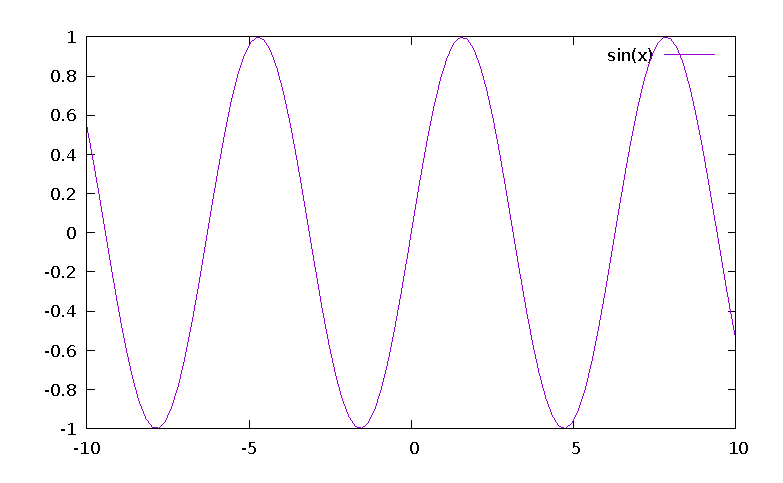
\includegraphics[width=0.5\textwidth]{F/sin}
    \caption{Graph of \(\sin(x)\).}
  \end{center}
\end{figure}




%%% Local Variables:
%%% mode: latex
%%% TeX-master: "paper"
%%% End:


\section[L and T]{\ifCDLeng Lemmas and Theorems\fi\ifCDLita Lemmi e Teoremi\fi}

\begin{Lem}[Cauchy]\label{lem:1}
  \lipsum[3]

  See \cite{wiki:it:tautol}
\end{Lem}

\begin{Theorem}[\ifCDLeng The main theorem\fi\ifCDLita Il teorema principale\fi]\label{thm:1}
  \CDLeng Using Definition
  \CDLita Usando la definizione
  \ref{defn:1} \\
  \lipsum[4]
  \begin{proof}
    \CDLeng Using 
    \CDLita Usando il Lemma \ref{lem:1}
    \begin{equation}
      \label{eq:1}
      {\mathbf{e}}^{i \pi }=-1
    \end{equation}
  \end{proof}
\end{Theorem}


\begin{Cor}\label{cor:1}
  \CDLeng Corollary to Theorem
  \CDLita Corollatio al Teorem
  \ref{thm:1}.
  \\
  \lipsum[6]
\end{Cor}

\begin{description}
  % a nasty comment
\item[one] 1
\item[two] 2 %due
\item[three] 3
\end{description}


%%% Local Variables:
%%% mode: latex
%%% TeX-master: "paper"
%%% End:


\section*{Table of contents}
\tableofcontents

\bibliographystyle{plain}
\bibliography{subdir/paper}

\end{document}
